\let\negmedspace\undefined
\let\negthickspace\undefined
\documentclass[journal]{IEEEtran}
\usepackage[a5paper, margin=10mm, onecolumn]{geometry}
\usepackage{lmodern} % Ensure lmodern is loaded for pdflatex
 % Include tfrupee package
\setlength{\headheight}{1cm} % Set the height of the header box
\setlength{\headsep}{0mm}     % Set the distance between the header box and the top of the text
\usepackage{enumitem}
\usepackage{gvv-book}
\usepackage{gvv}
\usepackage{cite}
\usepackage{amsmath,amssymb,amsfonts,amsthm}
\usepackage{algorithmic}
\usepackage{graphicx}
\usepackage{textcomp}
\usepackage{xcolor}
\usepackage{txfonts}
\usepackage{listings}
\usepackage{enumitem}
\usepackage{mathtools}
\usepackage{gensymb}
\usepackage{comment}
\usepackage[breaklinks=true]{hyperref}
\usepackage{tkz-euclide} 
\usepackage{listings}
% \usepackage{gvv}                                        
\def\inputGnumericTable{}                                 
\usepackage[latin1]{inputenc}                                
\usepackage{color}                                            
\usepackage{array}                                            
\usepackage{longtable}                                       
\usepackage{calc}                                             
\usepackage{multirow}                                         
\usepackage{hhline}                                           
\usepackage{ifthen}                                           
\usepackage{lscape}
\begin{document}

\bibliographystyle{IEEEtran}
\vspace{3cm}

\title{7-7.2-22}
\author{AI24BTECH11008- Sarvajith
}
% \maketitle
% \newpage
% \bigskip
{\let\newpage\relax\maketitle}

\renewcommand{\thefigure}{\theenumi}
\renewcommand{\thetable}{\theenumi}
\setlength{\intextsep}{10pt} % Space between text and floats
\numberwithin{equation}{enumi}
\numberwithin{figure}{enumi}
\renewcommand{\thetable}{\theenumi}
\textbf{Question: }\\
Find the equation of the circle having (1, -2) as its centre and passing through the
intersection of 3x + y = 14, 2x + 5y = 18.\\
\textbf{Solution: }\\
\renewcommand{\tablename}{TABLE 1}
\begin{table}[h!]    
\centering
 \begin{tabular}{|c|c|}
\hline
\textbf{lengths} & \textbf{values}\\
\hline
\textbf{BC} & 5.5cm\\
\hline
\textbf{AL} & 5.3cm\\
\hline
\end{tabular}

\caption{given values}
 \label{tab1-7-7.2-22-1}
\end{table}\\
Intersection point of the 2 linear equations $3x + y = 14$ and $2x + 5y = 18$ is given by\\
\begin{align*}
\myvec{3 & 1\\2 & 5}\myvec{x \\ y} = \myvec{14\\18}\\
\end{align*}
\begin{align*}
\myvec{3 & 1 & 14\\2 & 5 & 18}\xleftrightarrow[]{R_2 \leftarrow {3R_2-2R_1}}\myvec{3 & 1 & 14\\0 & 13 & 26}\\
\xleftrightarrow[]{R_2 \leftarrow {R_2/13}}\myvec{3 & 1 & 14\\0 & 1 & 2}\\
\xleftrightarrow[]{R_1 \leftarrow {R_1-R_2}}\myvec{3 & 0 & 12 \\0 & 1 & 2}\\
\xleftrightarrow[]{R_1 \leftarrow {R_1/3}}\myvec{1& 0 & 4\\0 & 1 & 2}\\
\end{align*}
$\therefore$ the intersecting point of the 2 lines is A(4,2).\\
\begin{align*}
	r = \norm{A-C} = \sqrt{\brak{A-C}^T\brak{A-C}} 
\end{align*}
Where A\brak{4,2} is point of intersection and point on the circle with the centre C\brak{1,-2}.
\begin{align*}
	r = \sqrt{\myvec{3 & 4}\myvec{3\\4}} = 5
\end{align*}
equation of a conic is given by  $x^TVx + 2u^Tx + f = 0$\\
 for a circle
\begin{align*}
 V &= \myvec{1&0\\0&1},\\ 
u&=\myvec{-h\\-k}, \\
f &= \norm{u}^2 - r^2\\
\end{align*}
substituting the above values in the equation we get 
\begin{align*}
x^Tx + 2\myvec{-1 & 2}x - 20 = 0
\end{align*}
\begin{figure}[h!]
\centering
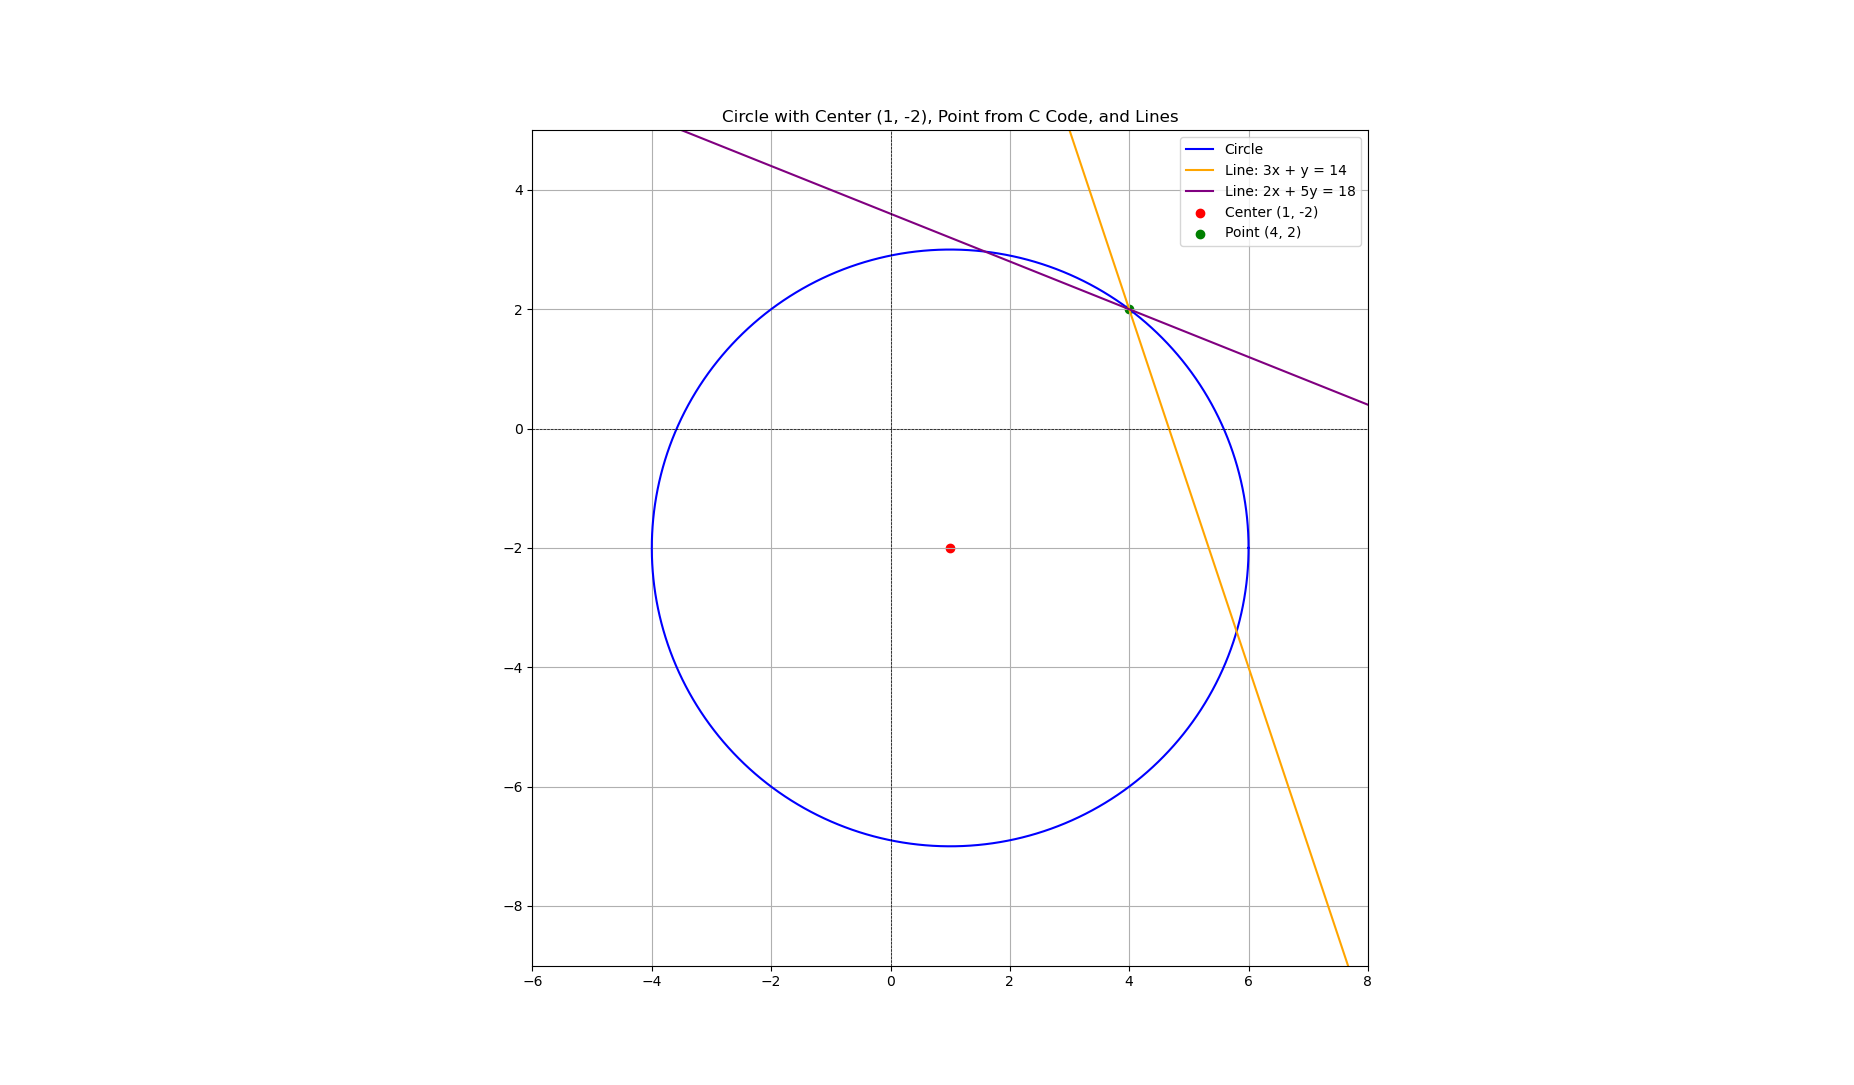
\includegraphics[width=0.7\columnwidth]{figs/Figure_1.png}
\caption{plot for circle}
 \label{fig. 7-7.2-22.1}
\end{figure}
\end{document}

